\documentclass[12pt]{article}
\usepackage{array}
\usepackage{float}
\usepackage{caption}
\usepackage{enumitem}
\usepackage{subcaption}
\usepackage[table, dvipsnames]{xcolor} 
\usepackage{graphicx}
\usepackage{longtable}
\usepackage{ltxtable}
\usepackage{wasysym}
\usepackage{tabularx}
\title{Project 50 Music Playlist Manager}
\date{}
\begin{document}
\maketitle
\noindent
\textbf{Team with Github names:}
\begin{itemize}[leftmargin=0.0cm,labelsep=0.2cm]
	\item[] Badam-Osor Khaltar (badamosor)
	\item[] Paul McCumber (paulmccumber)
	\item[] Luke Meszar (lukemeszar)
\end{itemize}
\textbf{Vision:} Provide a platform for building and sharing music playlists.
\section{Project Description}
Sharing playlists of music between a large group of people can be difficult when
everyone doesn't listen to music through the same service. This will allow people to create
playlists in a generic format that can then be integrated into the user’s service of choice. This allows people to share their playlists with their friends who can then export it into the streaming service of their choice. 
\section{Completed Requirements}
\rowcolors{2}{blue!10}{white}
\begin{table}[H]
	\centering
	\label{tab:urc}
	\caption*{User Requirements}
	\begin{tabularx}{450pt}{lXl}
		ID & Description & Priority\\\hline
		UR-01 & Users can create account & High \\
		UR-02 & Users can create a playlist & High \\
		UR-03 & Users can search database for song title, album title,
		artist, and playlist name & High \\
		UR-04 & Users can add content (songs, from albums or artists) to a playlist (only songs can be added) & High \\
		UR-06 & Users can make playlists collaborative & Low \\
		UR-07 & Users can share a playlist & High \\
		UR-11 & Users can export playlists into Spotify (through a fake API backend) & High \\
		UR-12 & Users can export playlists into Tidal (through a fake API backend) & High \\
		UR-13 & Users can export playlists into Google Play Music (through a fake API backend) & High \\
	\end{tabularx}
\end{table}
\begin{table}[H]
	\centering
	\label{tab:nfrc}
	\caption*{Non-Functional Requirements}
	\begin{tabularx}{450pt}{lXl}
		ID & Description & Priority\\\hline
		NFR-01 & Search has to be less than 20ms & High \\
		NFR-03 & Should be able to expand to other music services easily & Medium \\
	\end{tabularx}
\end{table}
\LTXtable{450pt}{functionalTableCompleted}
\section{Incomplete Requirements}
\rowcolors{2}{blue!10}{white}
\begin{table}[H]
	\centering
	\label{tab:uri}
	\caption*{User Requirements}
	\begin{tabularx}{450pt}{lXl}
		ID & Description & Priority\\\hline
		UR-05 & Users can remove songs from a playlist & Medium \\
		UR-08 & Users can register their Spotify account to our service & High \\
		UR-09 & Users can register their Tidal account to our service & High \\
		UR-10 & Users can register their Google Play Music account to our service & High \\
	\end{tabularx}
\end{table}
\begin{table}[H]
	\centering
	\label{tab:nfri}
	\caption*{Non-Functional Requirements}
	\begin{tabularx}{450pt}{lXl}
		ID & Description & Priority\\\hline
		NFR-02 & Service should support thousands of concurrent users & High \\
	\end{tabularx}
\end{table}
\LTXtable{450pt}{functionalTableIncomplete}
\section{Class Diagram}
\begin{figure}[H]
	\centering
	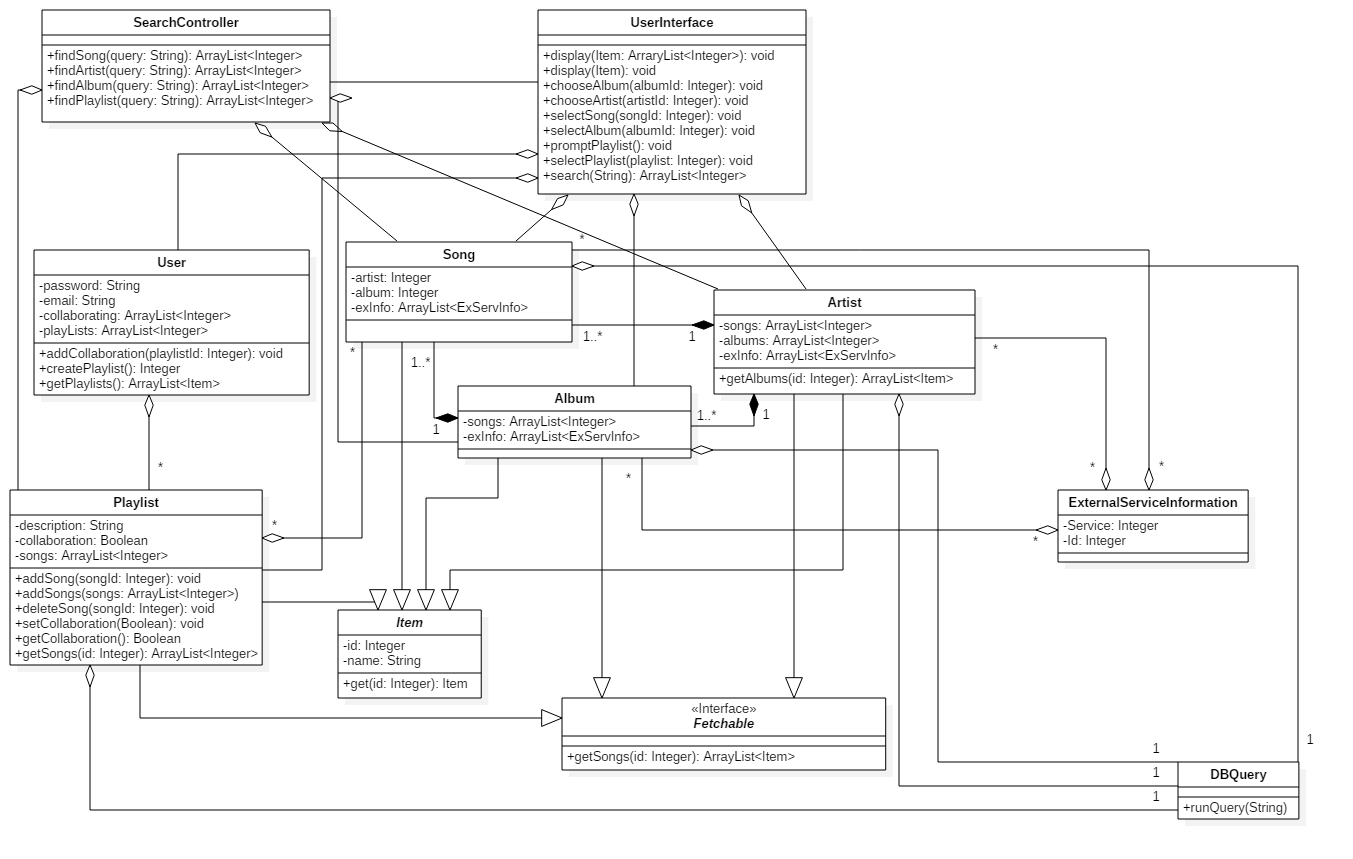
\includegraphics[scale=0.35]{MusicManagerClassDiagram.png}
	\caption{Class Diagram from Part 2}
	\label{fig:classDiagPart2}
\end{figure}
\begin{figure}[H]
	\centering
	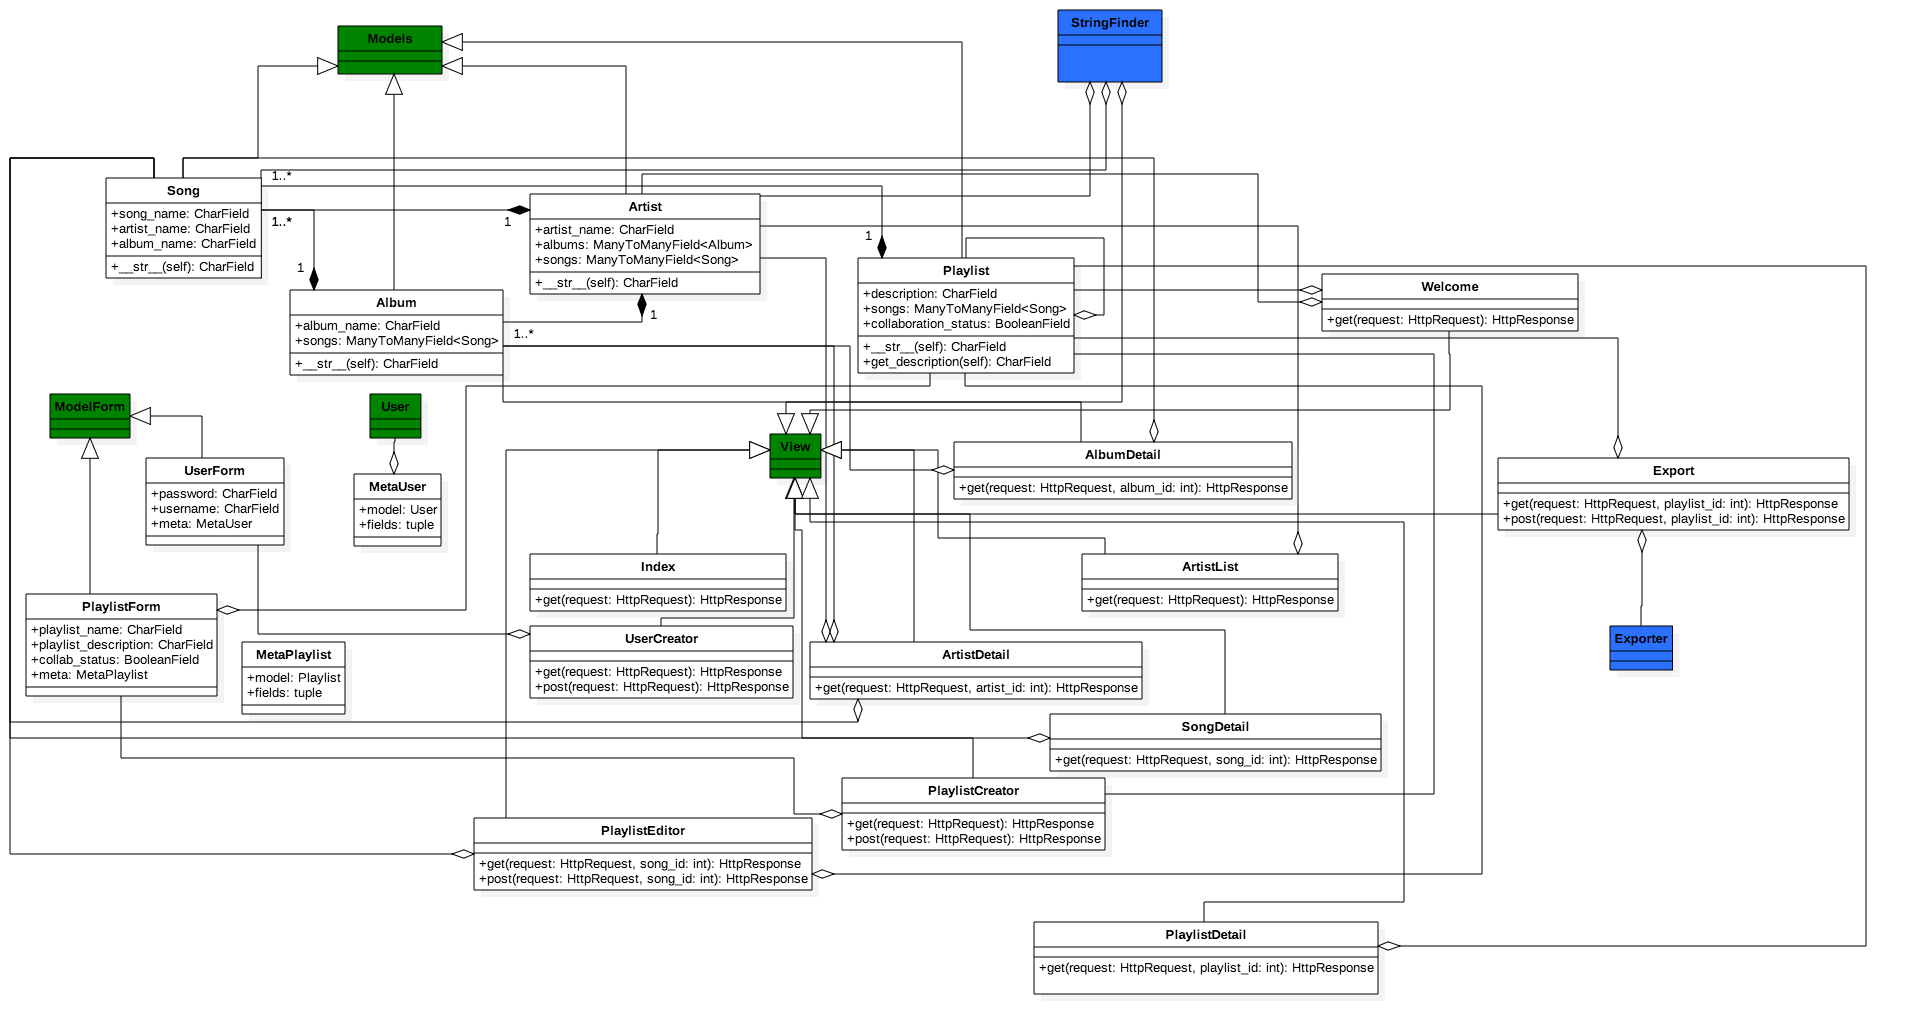
\includegraphics[scale=0.25]{DiagramAddedSearch.png}
	\caption{Class Diagram}
	\label{fig:classDiagCompleted}
\end{figure}
Our class diagram changed significantly between Part 2 and now. The fundamental reason for this is we started working with the Django framework after we finished the Part 2 
\end{document}